\documentclass{article}
\usepackage{tikz}
\usepackage{pgfplots}

\begin{document}

\begin{center}
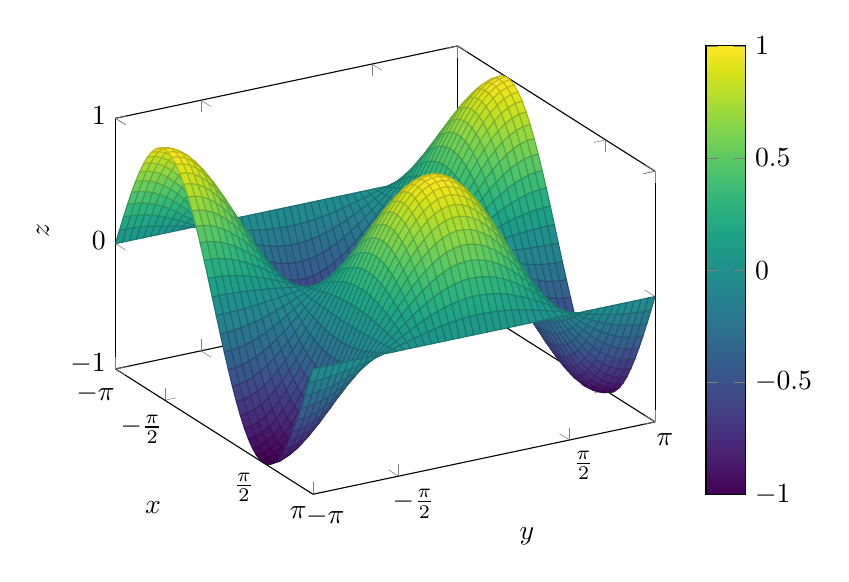
\begin{tikzpicture}
\begin{axis}[
    view={60}{30},
    xlabel=$x$,
    ylabel=$y$,
    zlabel=$z$,
    xmin=-pi,
    xmax=pi,
    ymin=-pi,
    ymax=pi,
    zmin=-1,
    zmax=1,
    xtick={-3.1416, -1.5708, 1.5708, 3.1416},
    xticklabels={$-\pi$, $-\frac{\pi}{2}$, $\frac{\pi}{2}$, $\pi$},
    ytick={-3.1416, -1.5708, 1.5708, 3.1416},
    yticklabels={$-\pi$, $-\frac{\pi}{2}$, $\frac{\pi}{2}$, $\pi$},
    ztick={-1, 0, 1},
    zticklabels={$-1$, $0$, $1$},
    colormap/viridis,
    colorbar
]
\addplot3[surf, domain=-pi:pi, samples=50, shader=faceted] {sin(deg(x))*cos(deg(y))};
\end{axis}
\end{tikzpicture}
\end{center}

\end{document}